% Emacs settings: -*-mode: latex; TeX-master: "manual.tex"; -*-

\chapter{Instrument examples}
\label{s:instrument}

Here, we give a short description of three selected
instruments. We present the \MCS\ versions of
the Ris\o\ standard triple axis spectrometer TAS1 (\ref{s:TAS1})
and the ISIS time-of-flight spectrometer PRISMA (\ref{s:PRISMA}).
Before that, however, we present one example of a component
test instrument: the instrument to test the component
{\bf V\_sample} (\ref{s:V-instr}).
%
%The source text for the three instrument definitions
%is listed in Appendix~\ref{instcode}.
These instrument files are included in the \MCS\ distribution
in the \verb+examples/+ directory.
It is also our intention to extend the list of instrument examples extensively
and perhaps publish them in a separate report.

\section{A test instrument for the component V\_sample}
\label{s:V-instr}
This instrument is one of many test instruments written with the
purpose of testing the individual components. We have picked 
this instrument both because we would like to present an
example test instrument and because it despite its simplicity
has produced quite non-trivial results, also giving rise to 
the \MCS\ logo.%, see Appendix~\ref{testresults}.

The instrument consists of a narrow source, 
a 60' collimator, a V-sample shaped as a hollow cylinder
with height 15 mm, inner diameter 16 mm, and outer diameter 24 mm
at a distance of 1 m from the source. 
The sample is in turn surrounded by an unphysical $4\pi$-PSD
monitor with $50 \times 100$ pixels and a radius of $10^{6}$ m. 
The set-up is shown in figure~\ref{f:V-instr}.

\begin{figure}
  \begin{center}
    \psfrag{Source}{Source}
    \psfrag{Collimator}{Collimator}
    \psfrag{Vanadium}{Vanadium}
    \psfrag{4pipsd}{$4\pi$ PSD}
    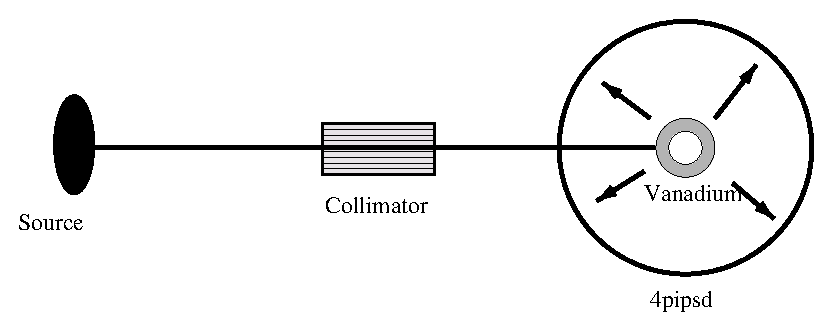
\includegraphics[width=0.9\textwidth]{figures/vanadium.eps}
  \end{center}
\caption{A sketch of the test instrument for the component
V\_sample.}
\label{f:V-instr}
\end{figure}

\subsection{Scattering from the V-sample test instrument}
\label{s:vanadium-result}

In figure \ref{f:V-results}, we present the radial distribution 
of the scatting from an evenly illuminated V-sample,
as seen by a spherical PSD.
It is interesting to note that the variation in the
scattering intensity is as large as 10\%. This is an effect
of attenuation of the beam in the cylindrical sample.

\begin{figure}
  \begin{center}
    \includegraphics[width=0.6\textwidth]{figures/vanadium-surf-2.eps}
  \end{center}
\caption{Scattering from a V-sample, measured by a spherical
  PSD. The sphere has been transformed onto a plane and the intensity is
  plotted as the third dimension. A colour version of this picture is
  found on the title page of this manual.}
\label{f:V-results}
\end{figure}



\section{The triple axis spectrometer TAS1}
\label{s:TAS1}
With this instrument definition, we have tried to create
a very detailed model of the conventional cold-source
triple-axis spectrometer TAS1 at Ris\o\ National Laboratory.
Unfortunately, no neutron scattering is performed at Ris\o\
anymore, but it still serves as a good example.
Except for the cold source itself, all components 
used have quite realistic properties. Furthermore, the overall
geometry of the instrument has been adapted from
the detailed technical drawings of the real spectrometer.
The TAS 1 simulation is the first detailed work
performed with the \MCS\ package.%, and a few of the simulation
%results are shown in Appendix \ref{testresults}.
For further details see reference~\cite{tas1_report}.

At the spectrometer, the channel from the cold source 
to the monochromator is asymmetric, since the first
part of the channel is shared with other instruments.
In the instrument definition, this is represented by
three slits.
For the cold source, we use a flat energy
distribution (component {\bf Source\_flat}) 
focusing on the third slit.

The real monochromator consist of seven blades, vertically focusing on
the sample. The angle of curvature is constant so that the focusing is
perfect at 5.0 meV (20.0 meV for 2nd order reflections) for a 1$\times$1~cm$^2$
sample. This is modeled directly in the instrument definition using
seven {\bf Monochromator} components. The mosaicity of the pyrolytic
graphite crystals is nominally 30' (FWHM) in both directions.  However, the
simulations indicated that the horisontal mosaicities of both
monochromator and analyser were more likely 45'. This was used for all
mosaicities in the final instrument definition.

The monochromator scattering angle, in effect determining the incoming
neutron energy, is for the real spectrometer fixed by four holes in the
shielding, corresponding to the energies 3.6, 5.0, 7.2, and 13.7~meV for
first order neutrons.  In the instrument definition, we have adapted the
angle corresponding to 5.0~meV in order to test the simulations against
measurements performed on the spectrometer.

The exit channel from the monochromator may 
on the spectrometer be narrowed down from initially 40~mm
to 20~mm by an insert piece. In the simulations, we have chosen
the 20~mm option and modeled the channel with two slits to match
the experimental set-up.

In the test experiments, we used two standard samples:
An Al$_2$O$_3$ powder sample and a vanadium sample. The instrument
definitions use either of these samples of the correct
size. Both samples are chosen to focus on the opening aperture of
collimator 2 (the one between the sample and the analyser).
Two slits, one before and one after the sample,
are in the instrument definition set to the opening values which
were used in the experiments.

The analyser of the spectrometer is flat and made from 
pyrolytic graphite. It is placed between an entry and 
an exit channel, the latter leading to a single detector.
All this has been copied into the instrument definition,
where the graphite mosaicity has been set to 45'.

On the spectrometer, Soller collimators may be inserted
at three positions: Between monochromator and sample,
between sample and analyser, and between analyser and detector.
In our instrument definition, we have used 30', 28', and 67' collimators
on these three positions, respectively.

An illustration of the TAS1 instrument
is shown in figure~\ref{f:TAS1}.
Test results and data from the real spectrometer are shown
in Appendix~\ref{data:TAS1}. 

\begin{figure}
  \begin{center}
    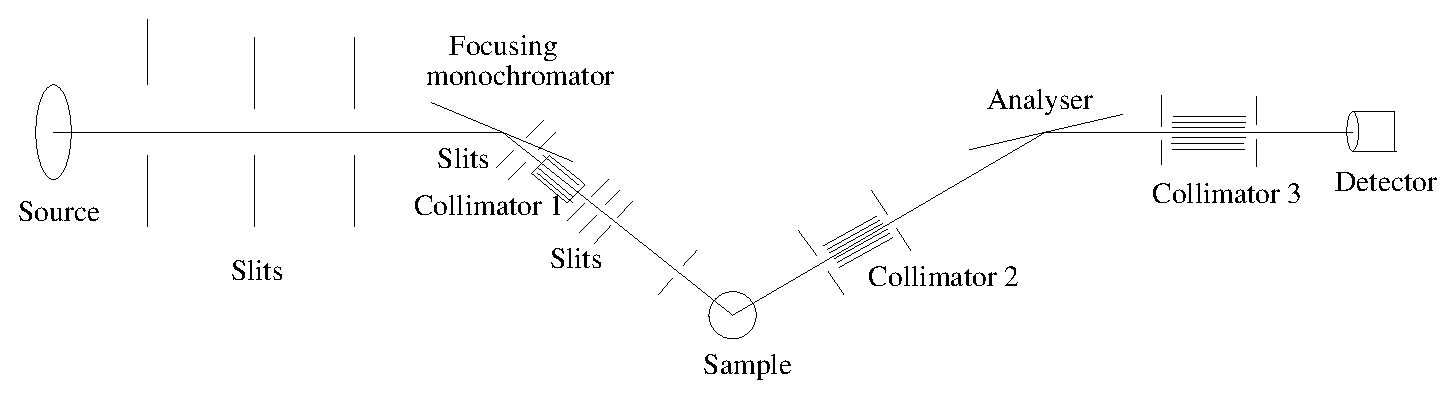
\includegraphics[width=0.9\textwidth]{figures/tas1.eps}
  \end{center}
\caption{A sketch of the TAS1 instrument.}
\label{f:TAS1}
\end{figure}

\subsection{Simulated and measured resolution of TAS1}
\label{data:TAS1}

In order to test the \MCS\ package on a qualitative level,
we have performed a very detailed simulation of the conventional
triple axis spectrometer TAS1, Ris\o . The measurement series
constitutes a complete alignment of the spectrometer,
using the direct beam and scattering from V and Al$_2$O$_3$
samples at an incoming energy of 20.0~meV, using the second order
scattering from the monochromator. 
In the instrument definitions, we have used all available
information about the spectrometer. However, the
mosaicities of the monochromator and analyser are set
to 45' in stead of the quoted 30', since we from our
analysis believe this to be much closer to the truth.

In these simulations, we have tried to reproduce
every alignment scan with respect to position and width
of the peaks, whereas we have not tried to compare
absolute intensities. Below, we show a few comparisons 
of the simulations and the measurements. 

Figure \ref{f:2t_direct} shows a scan of 
$2\theta_s$ on the collimated direct beam in two-axis mode.
A 1 mm slit is placed on the sample position.
Both the measured width and non-Gaussian peak shape
are well reproduced by the \MCS\ simulations.

\begin{figure}
  \begin{center}
    \includegraphics[width=0.6\textwidth]{figures/tas1-2T.eps}
  \end{center}
\caption{Scans of $2\theta_s$ in the direct beam with 1 mm slit on the
  sample position.
"$\times$": measurements, "o": simulations  
Collimations: open-30'-open-open.}
\label{f:2t_direct}
\end{figure}

In contrast, a simulated $2\theta_a$ scan in triple-axis 
mode on a V-sample showed a surprising offset from zero, see
Figure \ref{f:v_2ta_offset}. However, a simulation with a PSD
on the sample position showed that the beam center was 1.5~mm
off from the center of the sample, and this was important
since the beam was no wider than the sample itself.
A subsequent centering of the beam resulted in a nice
agreement between simulation and measurements. 
For a comparison on a slightly different instrument
(analyser-detector collimator inserted), 
see Figure~\ref{f:v_2ta_zero}.

\begin{figure}
  \begin{center}
    \includegraphics[width=0.6\textwidth]{figures/vanadium-plot-1.eps}
  \end{center}
\caption{First simulated $2\theta_a$ scan on a vanadium sample.
Collimations: open-30'-28'-open.}
\label{f:v_2ta_offset}
\end{figure}

\begin{figure}
  \begin{center}
    \includegraphics[width=0.6\textwidth]{figures/vanadium-plot-2.eps}
  \end{center}
\caption{Corrected $2\theta_a$ scan on a V-sample.
Collimations: open-30'-28'-67'.
"$\times$": measurements, "o": simulations.}
\label{f:v_2ta_zero}
\end{figure}

The result of a $2\theta_s$ scan on an Al$_2$O$_3$
powder sample in two-axis mode is shown in Figure \ref{f:al2o3}.
Both for the scan in focusing mode (+ $-$ +)
and for the one in defocusing mode (+ + +) (not shown),
the agreement between simulation and experiment is excellent.

\begin{figure}
  \begin{center}
    \includegraphics[width=0.6\textwidth]{figures/al2o3-focus.eps}
  \end{center}
\caption{$2\theta_s$ scans on Al$_2$O$_3$ in two-axis, focusing mode.
Collimations: open-30'-28'-67'.
"$\times$": measurements, "o": simulations.  
A constant background is added to the simulated data.}
\label{f:al2o3}
\end{figure}

As a final result, we present a scan of the energy
transfer $E_a = \hbar \omega$ on a V-sample.
The data are shown in Figure \ref{f:v_ea}.

\begin{figure}
  \begin{center}
    \includegraphics[width=0.6\textwidth]{figures/ea-scan.eps}
  \end{center}
\caption{Scans of the analyser energy on a V-sample.
Collimations: open-30'-28'-67'.
"$\times$": measurements, "o": simulations.}
\label{f:v_ea}
\end{figure}


\section{The time-of-flight spectrometer PRISMA}
\label{s:PRISMA} 

In order to test the time-of-flight aspect of \MCS, we have
in collaboration with Mark Hagen, ISIS, written a simple
simulation of a time-of-flight instrument loosely based on the ISIS
spectrometer PRISMA. The simulation was used to investigate the effect
of using a RITA-style analyser instead of the normal PRISMA backend.

We have used the simple time-of-flight source {\bf Tof\_source}. 
The neutrons pass through a
beam channel and scatter off from a vanadium sample, pass through
a collimator on to the analyser.
The RITA-style analyser consists of seven analyser crystals
that can be rotated independently around a vertical axis. After the
analysers we have placed a PSD and a time-of-flight detector.

To illustrate some of the things that can be done in a simulation as
opposed to a real-life experiment, this example instrument further
discriminates between
the scattering off each individual analyser crystal 
when the neutron hits the detector. The
analyser component is modified so that a global variable 
\verb+neu_color+ keeps track of which
crystal scatters the neutron. The detector component
is then modified to construct seven different time-of-flight histograms,
one for each crystal (see the source code for the instrument  
for details). One way to think of this is that
the analyser blades paint a color on each neutron which is then
observed in the detector.
An illustration of the instrument is shown in figure~\ref{f:PRISMA}.
Test results are shown in Appendix~\ref{data:PRISMA}.

\begin{figure}[h]
  \begin{center}
    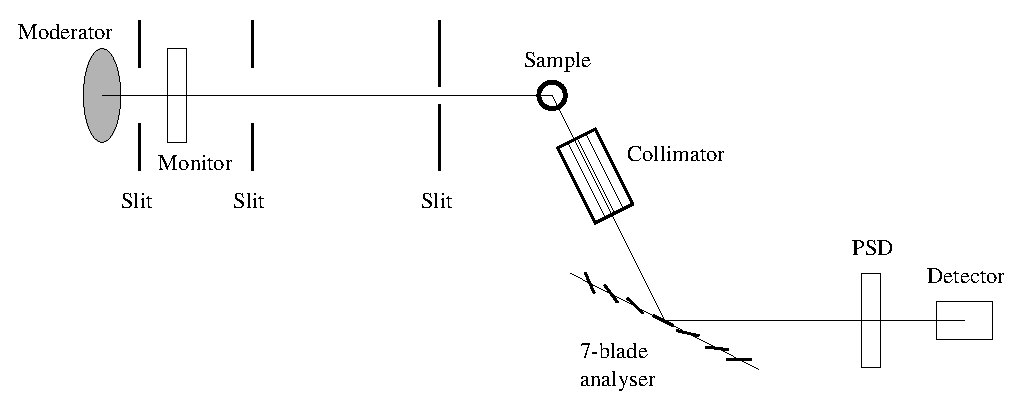
\includegraphics[width=0.9\textwidth]{figures/prisma2.eps}
  \end{center}
\caption{A sketch of the PRISMA instrument.}
\label{f:PRISMA}
\end{figure}

\subsection{Simple spectra from the PRISMA instrument}
\label{data:PRISMA}

A plot from the detector in the PRISMA simulation is shown in Figure
\ref{f:PRISMAdata}. These results were obtained with each analyser blade
rotated one degree relative to the previous one. The separation of the
spectra of the different analyser blades is caused by different energy
of scattered neutrons and different flight path length from source to
detector.  We have not performed any quantitative analysis of the data at this
time.

\begin{figure}
  \begin{center}
    \includegraphics[width=0.6\textwidth]{figures/prisma2-a.eps}
  \end{center}
\caption{Test result from PRISMA instrument using ``coloured
  neutrons''. Each graph shows the neutrons scattered from one analyser blade.}
\label{f:PRISMAdata}
\end{figure}
